\documentclass[12pt,letterpaper]{article}
\usepackage[utf8]{inputenc}
\usepackage[spanish, es-tabla]{babel}
\usepackage[version=3]{mhchem}
\usepackage[journal=jacs]{chemstyle}
\usepackage{amsmath}
\usepackage{amsfonts}
\usepackage{amssymb}
\usepackage{makeidx}
\usepackage{xcolor}
\usepackage[stable]{footmisc}
\usepackage[section]{placeins}
\usepackage{listings}
%Paquete para el manejo de las unidades
\usepackage{siunitx}
\sisetup{mode=text, output-decimal-marker = {,}, per-mode = symbol, qualifier-mode = phrase, qualifier-phrase = { de }, list-units = brackets, range-units = brackets, range-phrase = --}
\DeclareSIUnit[number-unit-product = \;] \atmosphere{atm}
\DeclareSIUnit[number-unit-product = \;] \pound{lb}
\DeclareSIUnit[number-unit-product = \;] \inch{"}
\DeclareSIUnit[number-unit-product = \;] \foot{ft}
\DeclareSIUnit[number-unit-product = \;] \yard{yd}
\DeclareSIUnit[number-unit-product = \;] \mile{mi}
\DeclareSIUnit[number-unit-product = \;] \pint{pt}
\DeclareSIUnit[number-unit-product = \;] \quart{qt}
\DeclareSIUnit[number-unit-product = \;] \flounce{fl-oz}
\DeclareSIUnit[number-unit-product = \;] \ounce{oz}
\DeclareSIUnit[number-unit-product = \;] \degreeFahrenheit{\SIUnitSymbolDegree F}
\DeclareSIUnit[number-unit-product = \;] \degreeRankine{\SIUnitSymbolDegree R}
\DeclareSIUnit[number-unit-product = \;] \usgallon{galón}
\DeclareSIUnit[number-unit-product = \;] \uma{uma}
\DeclareSIUnit[number-unit-product = \;] \ppm{ppm}
\DeclareSIUnit[number-unit-product = \;] \eqg{eq-g}
\DeclareSIUnit[number-unit-product = \;] \normal{\eqg\per\liter\of{solución}}
\DeclareSIUnit[number-unit-product = \;] \molal{\mole\per\kilo\gram\of{solvente}}
\usepackage{cancel}
%Paquetes necesarios para imágenes, pies de página, etc.
\usepackage{graphicx}
\usepackage{lmodern}
\usepackage{fancyhdr}
\usepackage[left=4cm,right=2cm,top=3cm,bottom=3cm]{geometry}

%Instrucción para evitar la indentación
%\setlength\parindent{0pt}
%Paquete para incluir la bibliografía
\usepackage[backend=bibtex,style=chem-acs,biblabel=dot]{biblatex}
\addbibresource{references.bib}

%Formato del título de las secciones

\usepackage{titlesec}
\usepackage{enumitem}
\titleformat*{\section}{\bfseries\large}
\titleformat*{\subsection}{\bfseries\normalsize}

%Creación del ambiente anexos
\usepackage{float}
\floatstyle{plaintop}
\newfloat{anexo}{thp}{anx}
\floatname{anexo}{Anexo}
\restylefloat{anexo}
\restylefloat{figure}

%Modificación del formato de los captions
\usepackage[margin=10pt,labelfont=bf]{caption}

%Paquete para incluir comentarios
\usepackage{todonotes}

%Paquete para incluir hipervínculos
\usepackage[colorlinks=true, 
            linkcolor = blue,
            urlcolor  = blue,
            citecolor = black,
            anchorcolor = blue]{hyperref}

%%%%%%%%%%%%%%%%%%%%%%
%Inicio del documento%
%%%%%%%%%%%%%%%%%%%%%%

\begin{document}
\renewcommand{\labelitemi}{$\checkmark$}

\renewcommand{\CancelColor}{\color{red}}

\newcolumntype{L}[1]{>{\raggedright\let\newline\\\arraybackslash}m{#1}}

\newcolumntype{C}[1]{>{\centering\let\newline\\\arraybackslash}m{#1}}

\newcolumntype{R}[1]{>{\raggedleft\let\newline\\\arraybackslash}m{#1}}

\begin{center}
	\textbf{\LARGE{Mineração de dados utilizando séries temporais}}\\
	\vspace{7mm}
	\textbf{\large{LaCCAN - Laboratório de computação científica e análise numérica}}\\ 
	\vspace{4mm}
	\textbf{\large{Aluna: Eduarda Chagas}}\\
	\vspace{4mm}
	\textbf{\large{Orientador: Alejandro Frery}}\\
\end{center}

\vspace{7mm}

\section*{\centering Resumo}

Este relatório possui como objetivo primordial relatar o processo de implementação de técnicas de mineração e pré-processamento de dados aplicados à análise de séries temporais.

Assim, primeiramente iremos apresentar uma breve introdução teórica a respeito da funcionalidade prática de cada código implementado, para logo após exibir o modo de funcionamento de cada uma delas. 

\section{Introdução}

Tendo como principal objetivo facilitar a análise de extensos volumes de dados, a mineração ou pré-processamento de dados vem simplificando este processo através de suas inovadoras técnicas, que possuem como característica reduzir substâncialmente o tamanho destes, porém mantendo intactas suas principais características.

Logo, com base nestas informações foram implementadas as seguintes técnicas: \textit{Piecewise aggregate approximation} (PAA), \textit{segmented sum of variation features}, \textit{perceptually important points} (PIP) e \textit{symbolic aggregate approximation} (SAX).

\section{Resultados}

\subsection{\textit{Piecewise aggregate approximation}}

Assim como as demais técnicas de mineração de dados, PAA também possui como objetivo reduzir a quantidade de dados que necessitam ser analisados pelo usuário. O método consiste em particionar a série em períodos igualitários e a partir disto calcular o valor médio dos dados de cada parte envolvida.\\

\textbf{Input :} Série temporal e o número de particionamentos.

\textbf{Output :} Um conjunto de dados representando a PAA.\\

\begin{lstlisting}
paa <- function(series,size){
  res = rep(0,size)
  for(i in 0:(length(series)*size-1)){
    res[i%/%length(series)+1] = res[i%/%length(series)+1] + series[i%/%size+1]
  }
  for(i in 1:size){
    res[i]=res[i]/length(series)
  }
  res
}
\end{lstlisting}

Por último foi implementada a função \textit{plotPAA} que possui como finalidade exibir gráficamente o resultado de tal técnica empregada na série temporal. Neste caso também será exibido para o usuário os valores correspondentes da função \textit{paa}.\\

\textbf{Input :} Série temporal e o número de particionamentos.

\textbf{Output :} O gráfico demonstrando o particionamento que foi realizado e os valores adquiridos após o cálculo da \textit{PAA}.\\

\begin{lstlisting}
plotPAA<-function(series,size,option=0){
  vline=seq(from=0,to=length(series),by=(length(series)/size))
  segm = rep(0,size+1)
  segm[1:size] = paa(series,size)
  segm[size+1] = segm[size]
  steps = data.frame(x=vline,y=segm)
  segm = as.double(format(round(segm,2),nsmall=2))
  myText = segm[1:size]
  p = qplot(x=c(1:length(series)),y=series,geom="line",xlab="Time",ylab="Serie",colour="red") +
      ggtitle("Piecewise Aggregate Approximation") + theme(plot.title = element_text(hjust=0.5)) +
      geom_step(data=steps,aes(x=x,y=y),colour="black") +
      geom_text(aes(x=(vline[1:(length(vline)-1)]+vline[2:length(vline)])/2,y=segm[1:(length(segm)-1)]*1.05,label=myText,colour="blue"))
  plot(p)
  print(segm[1:size])
}
\end{lstlisting}

\begin{figure}[!hbt]
	\begin{center}
		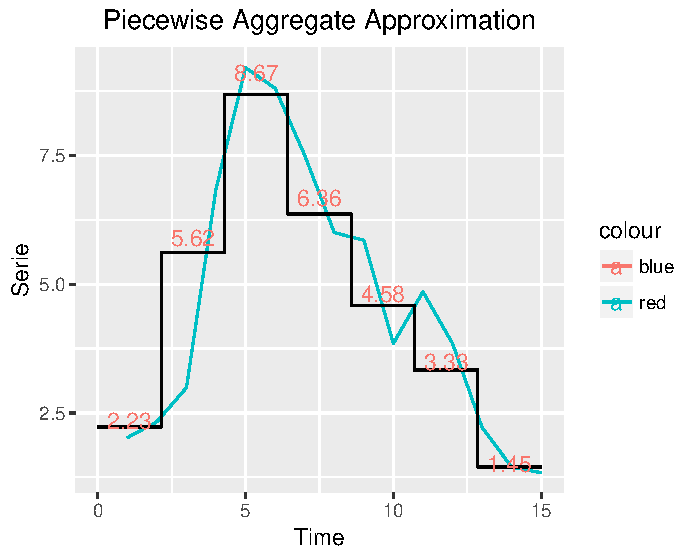
\includegraphics[width=\columnwidth]{PAA.pdf}
		\label{fig:PAA.pdf}
		\caption{Gráfico produzido pela função plotPAA ao utilizar a seguinte entrada de dados: series = c(2.02, 2.33, 2.99, 6.85, 9.20, 8.80, 7.50, 6.00, 5.85, 3.85, 4.85, 3.85, 2.22, 1.45, 1.34) e size = 7 }
	\end{center}
\end{figure}

Entretanto, quando o tamanho do particionamento é elevado foi diagnósticado problemas quanto a visualização dos valores correspondentes da PAA no gráfico, mas devido a este fato a função também é capaz de exibir estes valores separadamente.

\subsection{Função \textit{Segmented Sum of Variation Features}}

Muito utilizada como uma medida capaz de mensurar similaridades entre diferentes séries temporais, além de também ser uma importante técnica de redução da dimensão de dados, tal procedimento consiste dividir a série em segmentos de comprimento determinado anteriormente pelo usuário e assim calcular a soma variada de cada segmento desta.

Deste modo, para auxiliar tal processo foi implementada a função \textit{sum\underline{ }of\underline{ }variation}, que determinará a soma variada de cada parcela da série.\\

\textbf{Input :} Segmento da série, ou série.

\textbf{Output :} Soma variada da série fornecida.\\

 \begin{lstlisting}
sum_of_variation<-function(segment){
  c1 = segment[1:(length(segment)-1)]
  c2 = segment[2:length(segment)]
  res = sum(abs(c1-c2))
  res
}
\end{lstlisting}

E por último foi implementada a função responsável por particionar a série e calcular sua soma variada a partir da função descrita logo acima.\\

\textbf{Input :} Série temporal e o número de segmentos que esta deve possuir.

\textbf{Output :} Conjunto de dados contendo a soma variada de cada segmento da série.\\

 \begin{lstlisting}
ssv<-function(series,size){
  aux = matrix(nrow=round(length(series)/size),ncol=size)
  res = rep(0,round(length(series)/size))
  ini = row = sum = i = 1
  while((i <= length(series)) && (row <= round(length(series)/size))){
    aux[row,sum] = series[i]
    if(sum == size){
      row = row + 1
      sum = 1
      i = ini + size - 1
      ini = i
    }else{
      i = i + 1
      sum = sum + 1
    }
  }
  for(i in 1:round(length(series)/size)){
    res[i] = sum_of_variation(aux[i,])
  }
  res
}
\end{lstlisting}

\subsection{Função \textit{Perceptually Important Points}}

Definindo principais pontos de uma determinada série temporal, o algoritmo é capaz de encontrar quais dentres os fornecidos na série devem ser cogitados para que gráficamente a série preserve sua forma original, isto é quais são os pontos que mais representam a série.

Para identificar tais dados, o método considera inicialmente o primeiro e o último ponto da sequência como os seus dois mais importantes e a partir disto é calculado qual dentre os demais possui a menor ditância vertical entre a reta formada pelos dois pontos mencionados anteriormente. Após realizada a primeira etapa para encontrar os demais pontos é realizado todo o processo novamente, entretanto tendo como referência os três principais e as duas retas formadas por estes.

Logo o algoritmo implementado não apenas é capaz de encontrar tais pontos, como também plotar estes resultados e imprimir a sequência das posições dos tais pontos, pois ainda não sabemos um modo de como implementar corretamente o texto diante do gráfico, facilitando assim a leitura destes.\\

\textbf{Input :} A série temporal a ser analisada e número de pontos perceptivamente importantes.

\textbf{Output :} A posição dos pontos encontrados na série fornecida e a representação gráfica dos resultados.\\

\begin{lstlisting}
PIP<-function(serie,numberPIPs){ 
  pip=result=rep(0,numberPIPs) 
  texto = c(1:numberPIPs)
  x1 = pip[1] = result[1] = 1
  x2 = pip[2] = result[2] = length(serie)
  y1 = serie[x1]
  y2 = serie[x2]
  initial = 1 
  n = 2 
  p = qplot(x=c(1:length(serie)),y=serie,xlab="Time",ylab="Serie",colour="blue") +
      ggtitle("Perceptually Important Points") + theme(plot.title = element_text(hjust=0.5)) +
      geom_line(aes(x=c(1:length(serie)),y=serie))
  for(i in 3:numberPIPs){
    pip[1:n] = sort(pip[1:n])
    dis = rep(0,length(serie))
    x1 = pip[initial]
    y1 = serie[x1]
    x2 = pip[initial+1]
    y2 = serie[x2]
    for(j in 1:(length(serie))){
      x3 = j
      y3 = serie[x3]
      dis[j] = abs((y1 + (y2 - y1)*((x3-x1)/(x2-x1))) - y3)
      if(dis[j] == max(dis)){
        pip[n+1] = j
      }
      if(j == x2){
        if(j != length(serie)){
          initial = initial + 1 
          x1 = pip[initial]
          y1 = serie[x1]
          x2 = pip[initial+1]
          y2 = serie[x2]
        }
      }
    }
    n = n + 1
    initial = 1
    result[n] = pip[n]
  }
  pip = sort(pip)
  p = p + geom_line(aes(x=pip,y=serie[pip]),colour="red") +
      geom_text(aes(x=pip,y=serie[pip]*1.1,label=texto,colour="black"))
  plot(p)
  result 
}
\end{lstlisting}

\begin{figure}[!hbt]
	\begin{center}
		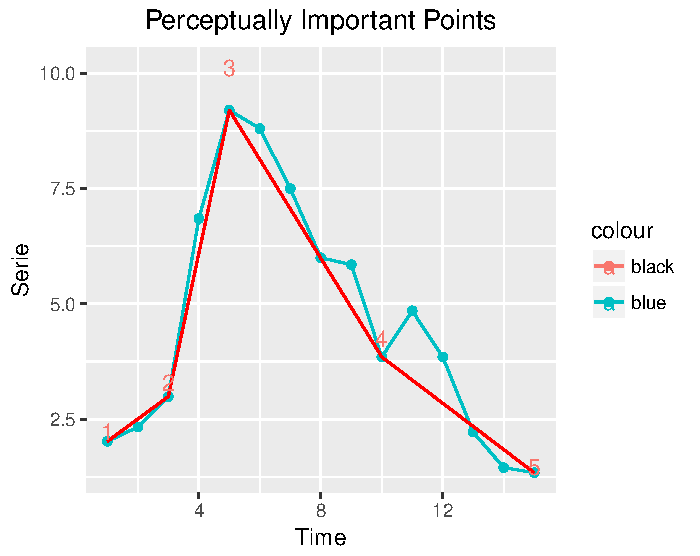
\includegraphics[width=\columnwidth]{PIP.pdf}
		\caption{Gráfico produzido pela função PIP ao utilizar a seguinte entrada de dados: serie = c(2.02, 2.33, 2.99, 6.85, 9.20, 8.80, 7.50, 6.00, 5.85, 3.85, 4.85, 3.85, 2.22, 1.45, 1.34) e numberPIPs = 5 }
		\label{fig:PIP.pdf}
	\end{center}
\end{figure}

\subsection{Função \textit{Symbolic Aggregate Approximation}}

Utilizando boa parte da metodologia utilizada na PAA, tal técnica consiste em calcular o PAA da série fornecida após esta ser normalizada e então classificar os valores adquiridos utilizando um conjunto de letras e valores da curva gaussiana.

Assim, após a série ser normalizada e ser encontrado seu PAA são encontrados os valores gaussianos que iram determinar a classificação da sequência. Logo, foram implementadas as funções \textit{lookupTable}, responsável por ler os valores gaussianos utilizados na análise e \textit{breakpoints} que possui a finalidade de retirar da função anterior a quantidade de dados que serão necessários para realizar o algoritmo, uma vez que será informado pelo usuário com quantas letras a pesquisa será realizada.

Desse modo, para a primeira parte do processo foi implementada  a função \textit{zNormalization}, que como sua própia denominação sugere, visa retornar a série normalizada.\\

\textbf{Input :} Série temporal que será utilizada no processo.

\textbf{Output :} Série normalizada.\\

\begin{lstlisting}
zNormalization<-function(series){
  (series - mean(series))/sd(series)
}
\end{lstlisting}

\textbf{Função \textit{lookupTable}}\\

\textbf{Input :} Não possui.

\textbf{Output :} Matriz contendo os valores Gaussianos.\\

\begin{lstlisting}
lookupTable<-function(){
  lookup=unlist(read.table("lookupTable.txt"))
  matrix(lookup,nrow=9,byrow=T)
}
\end{lstlisting}

\textbf{Função \textit{breakpoints}}\\

\textbf{Input :} O número de letras que serão utilizadas no procedimento, podendo tal número varia de 3 a 10.

\textbf{Output :} Valores Gaussianos solicitados de acordo com a entrada.\\

\begin{lstlisting}
breakpoints<-function(numberSymbols){
  numberSymbols = numberSymbols - 2
  lookup = lookupTable()
  na.omit(lookup[,numberSymbols])
}
\end{lstlisting}

E por último temos a função \textit{\textbf{saxPlot}} que será responsável por calcular a normalização da série (Através de uma chamada a outra função), calcular o PAA (Através de outra chamada de função) e a partir disto classificar tais valores. Tal implementação permite a representação gráfica dos resultados e imprime a string resultante da análise.\\

\textbf{Input :} A série temporal a ser considerada, o número de letras e o número de partições.

\textbf{Output :} A representação gráfica da análise e a string formada.\\

\begin{lstlisting}
saxPlot<-function(series,numberSymbols,size){
  letters = c("a","b","c","d","e","f","g","h","j","k")
  sax = ""
  series = zNormalization(series)
  segm = rep(0,size+1)
  Psax = rep(0,size)
  segm[1:size] = paa(series,size)
  segm[size+1] = segm[size]
  point = breakpoints(numberSymbols)
  for(i in 1:size){
    aux = 0
    for(j in 1:length(point)){ 
      if(segm[i] <= point[j]){
        sax = paste(letters[j],sax,sep="")
        Psax[i] = j
        aux = 1
        break
      }
    }
    if(!aux){ 
      sax = paste(letters[numberSymbols+1],sax,sep="")
      Psax[i] = numberSymbols+1
    }
  }
  steps = data.frame(x=vline,y=segm)
  p = qplot(geom="line",xlab="Time",ylab="Serie") +
    ggtitle("Symbolic Aggregate Approximation") + theme(plot.title = element_text(hjust=0.5)) +
    geom_hline(yintercept=point) + geom_step(data=steps,aes(x=x,y=y),colour="black") +
    geom_text(aes(x=(vline[1:(length(vline)-1)]+vline[2:length(vline)])/2,y=segm[1:(length(segm)-1)],label=letters[Psax],colour="red"))
  plot(p)
  print(sax)
}
\end{lstlisting}

\begin{figure}[!hbt]
	\begin{center}
		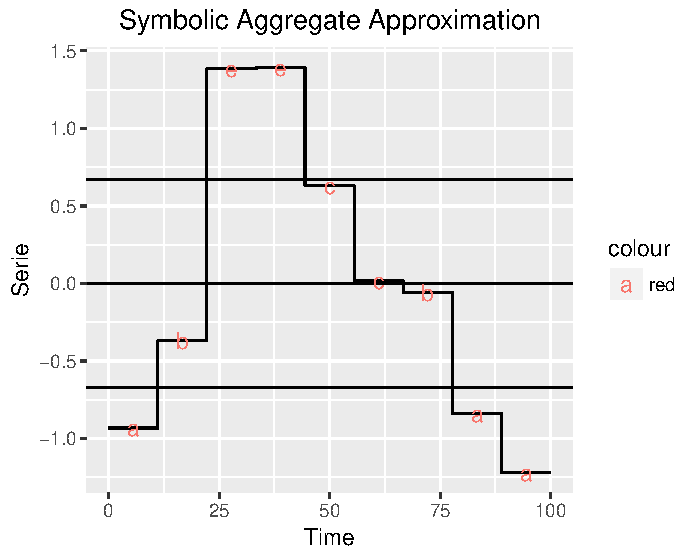
\includegraphics[width=\columnwidth]{SAX.pdf}
		\caption{Gráfico produzido pela função SAX ao utilizar a seguinte entrada de dados: series = c(2.02, 2.33, 2.99, 6.85, 9.20, 8.80, 7.50, 6.00, 5.85, 3.85, 4.85, 3.85, 2.22, 1.45, 1.34), numberSymbols = 4 e size = 9}
		\label{fig:SAX.pdf}
	\end{center}
\end{figure}

\section{Conclusões\label{conclusions}}

Desse modo, podemos perceber que a seção das funções implementadas de minaração de dados na análise de séries temporais foi devidamente implementada, contendo apenas um pequeno problema visual envolvendo a alocação de textos diante do gráfico. Também pode ser visto que o modo de implementação dos gráfico foi modificado, uma vez que para a codificação destes foi utilizado o pacote \textit{ggplot2}, que fornece melhores e mais sofisticadas ferramentas gráficas.

\end{document}
